\documentclass[tikz,border=6pt]{standalone}
\usepackage{amsmath,amssymb}
\usepackage{tikz}
\usetikzlibrary{arrows.meta,calc,decorations.pathreplacing,patterns,shapes.geometric,positioning,shadings,plotmarks}

\begin{document}
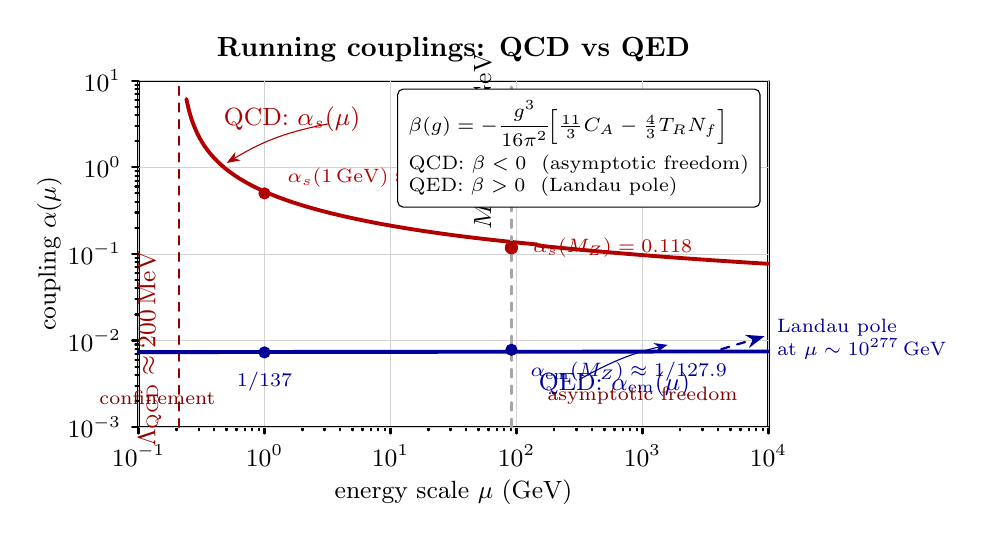
\begin{tikzpicture}[>=Stealth,line cap=round,line join=round]

% ---------------------------------------------------------------
% log-log axes:
%   x = log10(mu/GeV),   range [-1, 4]
%   y = log10(alpha),    range [-3, 1]
% scale: 1.6 cm per x-decade, 1.1 cm per y-decade
% ---------------------------------------------------------------
\def\xs{1.6}
\def\ys{1.1}

% --- Axis box ---
\draw[thick] (-1*\xs,-3*\ys) rectangle (4*\xs,1*\ys);

% --- Vertical gridlines (decades) and x labels ---
\foreach \xv/\lab in {-1/{$10^{-1}$},0/{$10^{0}$},1/{$10^{1}$},2/{$10^{2}$},3/{$10^{3}$},4/{$10^{4}$}}{
  \draw[gray!35,very thin] (\xv*\xs,-3*\ys) -- (\xv*\xs,1*\ys);
  \draw[thick] (\xv*\xs,-3*\ys) -- (\xv*\xs,{-3*\ys-0.08});
  \node[below,font=\small] at (\xv*\xs,{-3*\ys-0.10}) {\lab};
}
% minor x ticks
\foreach \xv in {-1,0,1,2,3}{
  \foreach \k in {2,3,4,5,6,7,8,9}{
    \pgfmathsetmacro{\xt}{\xv+ln(\k)/ln(10)}
    \draw[thick] (\xt*\xs,-3*\ys) -- (\xt*\xs,{-3*\ys-0.04});
  }
}

% --- Horizontal gridlines (decades) and y labels ---
\foreach \yv/\lab in {-3/{$10^{-3}$},-2/{$10^{-2}$},-1/{$10^{-1}$},0/{$10^{0}$},1/{$10^{1}$}}{
  \draw[gray!35,very thin] (-1*\xs,\yv*\ys) -- (4*\xs,\yv*\ys);
  \draw[thick] (-1*\xs,\yv*\ys) -- ({-1*\xs-0.08},\yv*\ys);
  \node[left,font=\small] at ({-1*\xs-0.10},\yv*\ys) {\lab};
}
% minor y ticks
\foreach \yv in {-3,-2,-1,0}{
  \foreach \k in {2,3,4,5,6,7,8,9}{
    \pgfmathsetmacro{\yt}{\yv+ln(\k)/ln(10)}
    \draw[thick] (-1*\xs,\yt*\ys) -- ({-1*\xs-0.04},\yt*\ys);
  }
}

% --- Axis labels ---
\node[below,font=\small] at ({1.5*\xs},{-3*\ys-0.55}) {energy scale $\mu$ (GeV)};
\node[rotate=90,above,font=\small] at ({-1*\xs-0.85},{-1*\ys}) {coupling $\alpha(\mu)$};

% ---------------------------------------------------------------
% QCD curve:  alpha_s(mu) = 4*pi / ( (11 - 2*5/3) * ln(mu^2/Lambda^2) )
%           = (12*pi)/23 / ln(mu^2/Lambda^2)    with Lambda = 0.21 GeV
% In log-log: x = log10(mu),  y = log10(alpha_s)
% Lambda corresponds to x = log10(0.21) approx -0.6778
% ---------------------------------------------------------------
\def\LamLog{-0.6778}   % log10(0.21)
\def\Cqcd{1.6388}      % 12*pi/23
% pole asymptote
\draw[red!55!black,thick,dashed] (\LamLog*\xs,-3*\ys) -- (\LamLog*\xs,1*\ys);

% draw QCD curve from x just above Lambda up to x=4
% sample many x in [-0.62, 4]; plot y = log10( C / ( 2*ln(10)*(x - LamLog) ) )
\draw[red!70!black,line width=1.4pt,smooth,samples=300,domain=-0.62:4]
  plot (\x*\xs, { ln( \Cqcd / ( 2*ln(10)*(\x - \LamLog) ) ) / ln(10) * \ys });

% ---------------------------------------------------------------
% QED curve (illustrative, fixed-N_f leading log):
%  alpha_em(mu) = alpha0 / ( 1 - (2 alpha0 / 3 pi) ln(mu/m_e) )
%  alpha0 = 1/137.036, m_e = 0.000511 GeV
% In log-log y = log10(alpha)
% Curve very nearly flat over our window; rises slowly toward high mu.
% ---------------------------------------------------------------
\def\LogMe{-3.292}   % log10(0.000511)
\def\Aqed{0.007297}  % 1/137.036
% draw QED curve as smooth interpolation
\draw[blue!60!black,line width=1.4pt,smooth,samples=200,domain=-1:4]
  plot (\x*\xs, { ln( \Aqed / ( 1 - (2*\Aqed/(3*pi)) * ln(10) * (\x - \LogMe) ) ) / ln(10) * \ys });

% Landau pole symbolic arrow at right edge (pole at ~10^277)
\draw[blue!60!black,->,thick,dashed] ({4*\xs - 0.6},{-2.10*\ys}) -- ({4*\xs - 0.05},{-1.95*\ys});
\node[blue!60!black,font=\scriptsize,right=1pt] at ({4*\xs - 0.05},{-1.85*\ys}) {Landau pole};
\node[blue!60!black,font=\scriptsize,right=1pt] at ({4*\xs - 0.05},{-2.10*\ys}) {at $\mu \sim 10^{277}\,\mathrm{GeV}$};

% ---------------------------------------------------------------
% Vertical reference lines: Lambda_QCD and M_Z
% ---------------------------------------------------------------
% Lambda_QCD label
\node[red!60!black,font=\small,rotate=90,anchor=south] at ({\LamLog*\xs - 0.10},{-2.1*\ys}) {$\Lambda_{\mathrm{QCD}} \approx 200\,\mathrm{MeV}$};

% M_Z line at log10(91.19) = 1.96
\def\MZlog{1.9600}
\draw[gray!70,thick,dashed] ({\MZlog*\xs},-3*\ys) -- ({\MZlog*\xs},1*\ys);
\node[font=\small,rotate=90,anchor=south] at ({\MZlog*\xs - 0.10},{0.30*\ys}) {$M_Z = 91.2\,\mathrm{GeV}$};

% ---------------------------------------------------------------
% Markers
% ---------------------------------------------------------------
% alpha_s(M_Z) = 0.118 -> log10 = -0.928
\filldraw[red!70!black] ({\MZlog*\xs},{-0.928*\ys}) circle (2.2pt);
\node[red!70!black,font=\scriptsize,right=2pt] at ({\MZlog*\xs+0.08},{-0.928*\ys}) {$\alpha_s(M_Z)=0.118$};

% alpha_s(1 GeV) ~ 0.5 -> log10 ~ -0.301
\filldraw[red!70!black] ({0*\xs},{-0.301*\ys}) circle (2.0pt);
\node[red!70!black,font=\scriptsize,right=2pt] at ({0*\xs+0.10},{-0.30*\ys + 0.20}) {$\alpha_s(1\,\mathrm{GeV})\approx 0.5$};

% alpha_em(M_Z) ~ 1/127.9 = 0.007819 -> log10 = -2.107
\filldraw[blue!60!black] ({\MZlog*\xs},{-2.107*\ys}) circle (2.0pt);
\node[blue!60!black,font=\scriptsize,below right=1pt and 2pt] at ({\MZlog*\xs+0.05},{-2.107*\ys}) {$\alpha_{\mathrm{em}}(M_Z)\approx 1/127.9$};

% alpha_em(0) = 1/137.036 -> log10 = -2.137
\filldraw[blue!60!black] ({0*\xs},{-2.137*\ys}) circle (2.0pt);
\node[blue!60!black,font=\scriptsize,below=2pt] at ({0*\xs},{-2.137*\ys-0.05}) {$1/137$};

% ---------------------------------------------------------------
% Curve labels
% ---------------------------------------------------------------
% QCD label near steep low-mu region
\node[red!70!black,font=\small,anchor=west] at ({-0.40*\xs},{0.55*\ys}) {QCD: $\alpha_s(\mu)$};
\draw[red!70!black,->,thin] ({0.50*\xs},{0.50*\ys}) to[bend right=10] ({-0.30*\xs},{0.05*\ys});

% QED label near right
\node[blue!60!black,font=\small,anchor=west] at ({2.10*\xs},{-2.50*\ys}) {QED: $\alpha_{\mathrm{em}}(\mu)$};
\draw[blue!60!black,->,thin] ({2.50*\xs},{-2.45*\ys}) to[bend left=8] ({3.20*\xs},{-2.05*\ys});

% ---------------------------------------------------------------
% Annotation box (top-right inside): beta-function signs
% ---------------------------------------------------------------
\node[draw,fill=white,rounded corners=2pt,inner sep=4pt,font=\scriptsize,
      align=left,anchor=north east]
  at ({4*\xs - 0.10},{1*\ys - 0.10})
  {$\beta(g) = -\dfrac{g^{3}}{16\pi^{2}}\!\Bigl[\tfrac{11}{3}C_A - \tfrac{4}{3}T_R N_f\Bigr]$ \\[2pt]
   QCD: $\beta < 0$ \ (asymptotic freedom) \\
   QED: $\beta > 0$ \ (Landau pole)};

% ---------------------------------------------------------------
% Region annotations
% ---------------------------------------------------------------
\node[font=\scriptsize,red!50!black,anchor=south] at ({-0.85*\xs},{-2.85*\ys}) {confinement};
\node[font=\scriptsize,red!50!black,anchor=south] at ({3.0*\xs},{-2.85*\ys}) {asymptotic freedom};

% Title
\node[font=\bfseries] at ({1.5*\xs},{1*\ys + 0.40}) {Running couplings: QCD vs QED};

\end{tikzpicture}
\end{document}
